\section{SYSTEM}\label{sec:system}

The system is built in seven layers (Figure~\ref{fig:arch}). Layers 1 and 2 form the data plane and
its telemetry, layer 3 holds the four bounded agents, layer 4 is the policy gate, and layer 5
executes and audits whatever the gate allows. Layers 6 and 7, orchestration and enterprise
governance, extend the base paper's design. The campaign exercised layers 1 through 4, the
write-ahead audit log in layer 5, and the control loop and arbitration in layer 6; it never
exercised the autonomy-mode transitions, never engaged the kill switch, and never used layer 7. The
rest of this section follows the layers in order.

\begin{figure*}[t]
\centering
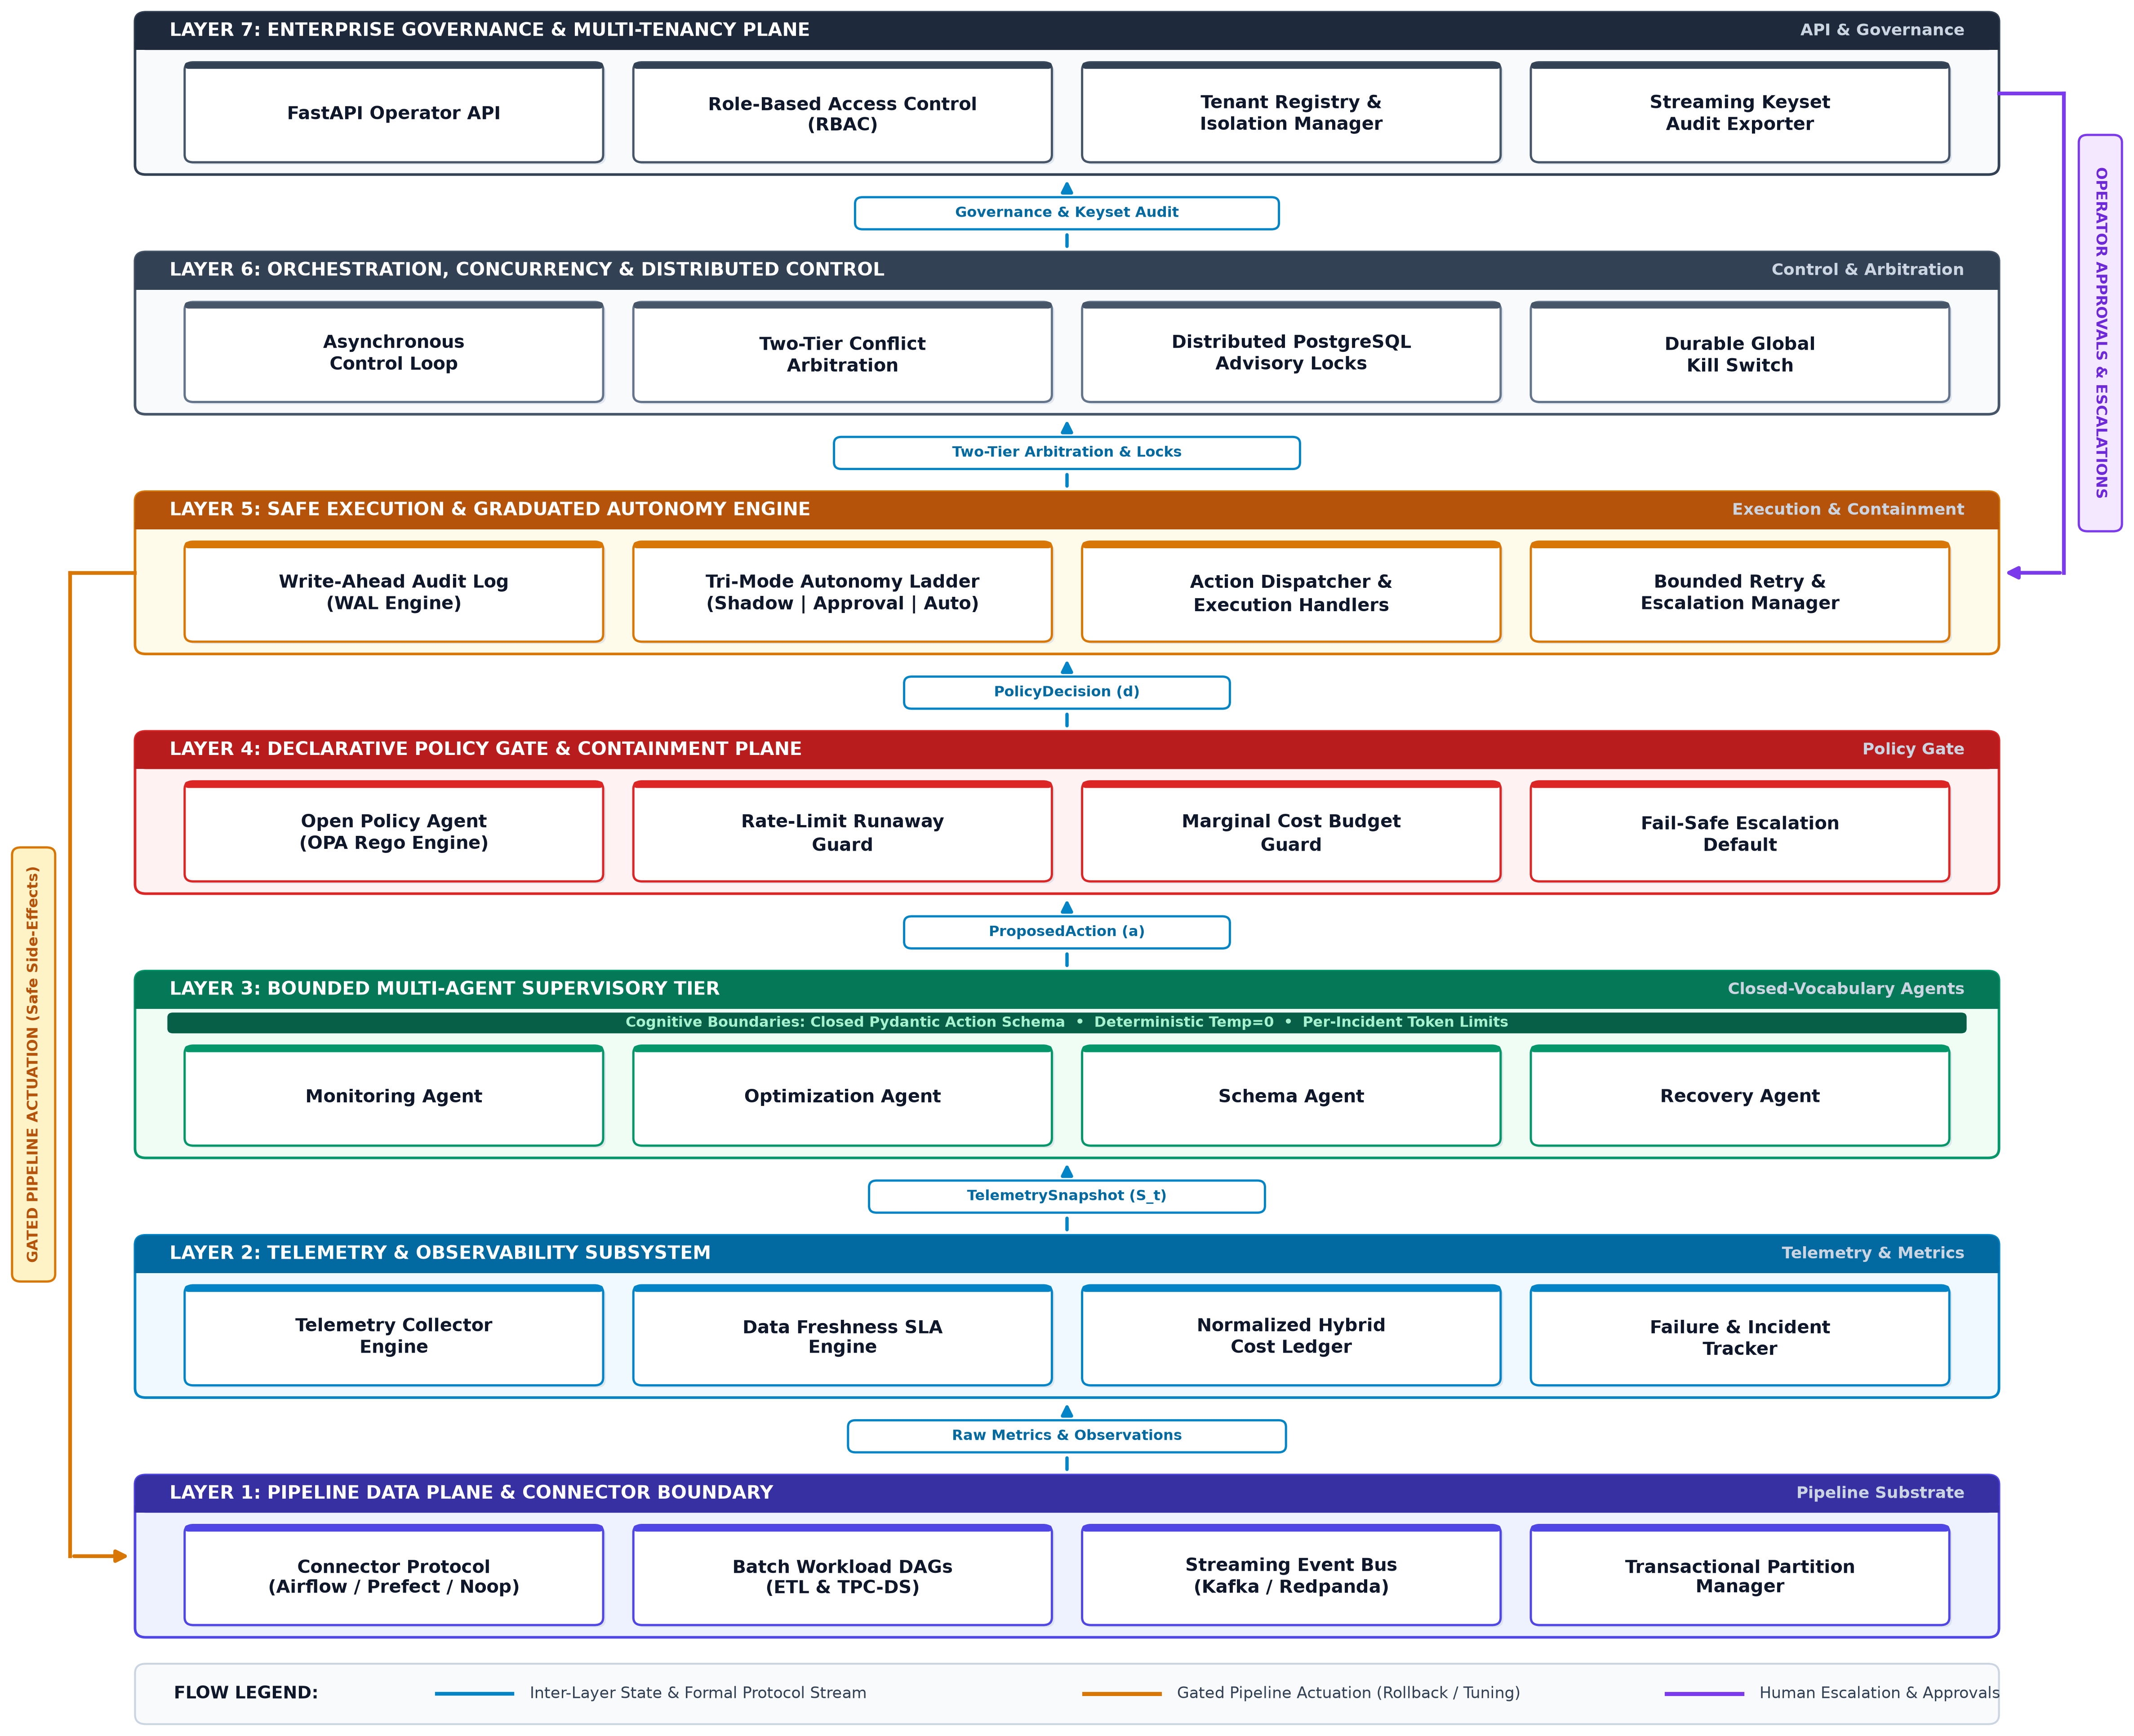
\includegraphics[width=\linewidth]{figures/system_architecture_7layer.png}
\caption{Seven-layer system architecture.}
\label{fig:arch}
\end{figure*}

\subsection{Layers 1 and 2: Data Plane and Telemetry}
A batch pipeline in Apache Airflow ingests a TPC-DS-derived dataset into versioned warehouse
partitions, while a streaming consumer reads from a Redpanda topic. All telemetry, pipeline metrics,
resource usage, task runs, agent actions, failure events, and manual interventions alike, lands in a
PostgreSQL \texttt{telemetry} schema, and every experimental metric in this paper is reconstructed
from that schema rather than logged separately. The same layer tracks data freshness and failure
events and keeps the cost ledger that backs the cost model of Eq.~\ref{eq:cost}.

\subsection{Layers 3 and 6: Agents and Orchestration}
Four agents share a single loop: \emph{observe} a telemetry snapshot, \emph{reason} with a live or
mock language model, \emph{propose}, and \emph{act}. Monitoring is the detector, enabled in every
non-baseline configuration so recovery time stays measurable in every ablation. Optimization scales
workers or pool slots, or reprioritizes work. Schema allows compatible changes and contains the
breaking ones. Recovery retries, replays, rolls back, partially recomputes, or escalates to a human.
When two proposals target the same resource, a static agent-priority bid settles the conflict rather
than lock ordering, since an earlier design that leaned on lock ordering for this property turned out
not to provide it; a per-target advisory lock still guards against a second process acting on the
same target.

\subsection{The Contract Between Layers 3 and 4}
An agent's only output is a \texttt{ProposedAction} carrying six fields: agent, action type, target,
parameters, justification, and confidence. A typed schema validates it, rejecting any action type
outside the agent's allowlist and any scaling target that is not an integer of at least one. That
second check exists because the adversarial corpus (Section~\ref{sec:results}) found it missing.
Invalid output is rejected, logged, and counted as \texttt{agent\_output\_invalid}, with the agent's
turn degrading to \texttt{no\_action}. Agents never emit or execute code.

\subsection{Layer 4: Policy Gate}
Every proposal carries a system-built context: projected marginal cost, remaining budget, the count
of actions taken in the last ten minutes, schema compatibility, and whether a prior version exists.
Four Rego policy packs evaluate it, namely a rate limit (Eq.~\ref{eq:rate}), a cost budget (Eq.~\ref{eq:budget}), a recovery-approval policy
that permits rollback only when a prior version exists, and a schema-compatibility policy. The
resulting decision is allow, deny, escalate, or allow-and-notify, and an unreachable policy engine
makes the gate escalate rather than allow by default.

\subsection{Layer 5: Execution and Audit}
An intent row is written and committed \emph{before} the executor runs and is updated with the
outcome afterward, so a crash mid-action leaves a durable \texttt{executing} row rather than no row
at all; this write-ahead ordering is a later fix, not part of the original design. An action
dispatcher then routes each allowed action type to a handler that carries out its side effect, on
Airflow by triggering DAG runs, clearing tasks, and patching pool slots, or on PostgreSQL by
rollback, quarantine, schema mapping, and desired-state updates.

\subsection{Simulated Human}
Escalations resolve after a seeded log-normal delay (median \NHumanMedian{}\,s,
$\sigma=\NHumanSigma{}$) standing in for the on-call engineer. This is a modeling choice rather than
a measurement, and Section~\ref{sec:sensitivity} quantifies how much the headline results lean on
it.

\subsection{Cross-Model Harness, Implemented but Not Evaluated}
A cross-model harness pushes a scenario through a configurable set of LLM backends and scores
decision correctness, latency, and tokens per model, a direct test of the base paper's
model-agnostic claim. The harness is unit-tested, but this campaign never ran or recorded the sweep
across real provider models, so no result from it appears here.

\subsection{Layers 5 and 6: Trust Core, Implemented but Not Evaluated}
Beyond the base paper's design, the system adds a graduated-autonomy layer with three modes.
\texttt{shadow} mode logs proposals without touching the pipeline; \texttt{approval} mode queues
allowed actions for a human decision; \texttt{autonomous} mode executes them outright. A durable kill
switch, checked once per control-loop tick, and a per-target hourly blast-radius cap bound the agents
independently of policy. Every mechanism is implemented and unit-tested, yet the campaign ran every
configuration in one fixed mode throughout, so this subsection describes capability, not something we
measured.

\subsection{Layer 7: Enterprise Governance, Implemented but Not Evaluated}
An operator API gives read access to proposals, the audit trail, and costs, and exports the full
audit log through a keyset cursor. Role-based access control, spanning viewer, approver, and admin
roles, together with a tenant registry, binds each actor to a tenant and lets an operator suspend
one. This layer supports multi-tenant deployment, but it played no part in the experimental
measurements.
